\documentclass[a4paper,onecolumn,10pt]{article}

\usepackage{geometry}
\geometry{a4paper,margin=3cm}
\usepackage[hybrid]{markdown}
\usepackage[scaled]{helvet}
%\usepackage{float}
\renewcommand\familydefault{\sfdefault}
\usepackage[T1]{fontenc}
\usepackage{pdfpages}
\usepackage{graphicx}
\usepackage{subfig}
\usepackage{float}
\usepackage[hidelinks, colorlinks=true, linkcolor=blue]{hyperref}
\usepackage[capitalise]{cleveref}

\usepackage{xurl}

\begin{document}


\title{Genomic projects}
\author{Stefano Scansani}
\date{\today}
\maketitle
\begin{abstract}

    The first project is about the high-density characterization of Durum wheat (\textit{Triticum turgidum} subsp. \textit{durum}).
    The second project is about a dataset of wild \textit{Vitis vinifera} subsp. sylvestris.
    The third and fourth projects are genomic tutorials on two animal studies, the first on worlwide populations of goats, the second on the association of deafness in three dog breeds.

\end{abstract}
\tableofcontents
\listoffigures
\listoftables


%\begin{twocolumn}
\section{Project: SNP Profiling of a Durum Wheat collection}

\subsection{Data}

Mengistu, D.K., Kidane, Y.G., Catellani, M., Frascaroli, E., Fadda, C., Pè, M.E. and Dell'Acqua, M. (2016), High-density molecular characterization and association mapping in Ethiopian durum wheat landraces reveals high diversity and potential for wheat breeding. Plant Biotechnol J, 14: 1800-1812. https://doi.org/10.1111/pbi.12538

The data used in this case study are derived from the durum wheat molecular characterization above-mentioned.
311 accessions of durum wheat were genotyped and phenotyped for some agronomic traits of interest.

The data are available in the DRYAD repository https://doi.org/10.5061/dryad.w6m905qrv.

For convenience, the abstract of the data accession is reported below:

\quote{
    \textit{<<Abstract: \\
        In smallholder, low-input farming systems diffused in the Global South, farmers select and propagate crop varieties based on their traditional knowledge and experience. A quantitative integration of their knowledge into breeding pipelines may support the sustainable intensification of local farming. This data entry combines genomics with socioeconomics to tap into traditional knowledge in smallholder farming systems, focusing on durum wheat (Triticum durum Desf.). Data refer to a large nested association mapping (EtNAM) population that we developed by recombining elite international breeding line with Ethiopian traditional varieties maintained by local farmers. This entry carries also molecular and phenotypic data produced on a diversity panel (DP) of Ethiopian landraces previously characterized in four year-location combinations and published in Mengistu et al 2016.\\
        EtNAM lines and DP genotypes were evaluated for agronomic performances and farmers’ appreciation in multiple locations, reveailing that gender and location can influence farmers’ preference and that women and men farmers can consistently identify the best durum wheat genotypes. We used this data to train a genomic selection (GS) model with farmer scores to show that their prediction accuracy over grain yield was higher than that of the benchmark GS model trained on grain yield. The data was also used in a genome wide association mapping (GWAS) and quantitative trait locus (QTL) mapping to identify genetic determinants of agronomic traits and farmer scores.  Our data shows that farmers’ traditional knowledge can be integrated in a quantitative framework to increase genetic gain in pre-breeding programs, supporting genomics-driven breeding for local adaptation.\\
        The Rdata files contain phenotypic and molecular characterization data for 1,200 recombinant inbred lines (RILs) deriving from the EtNAM and phenotypic and molecular characterization data for 400 durum wheat genotypes in the Ethiopian DP.>>}\\
    (Mengistu et al 2016 (https://doi.org/10.1111/pbi.12538).)
}

\subsection{Phenotype data}

In the Rdata \texttt{diversity.panel.data.gp.Rdata}, the agronomic traits of the population of Durum wheat (\textit{Triticum turgidum} subsp. \textit{durum}).

\subsubsection{Correlation between variables}

In \cref{fig:wheat_corr} the Pearson's correlation between agronomic traits is computed.

\begin{figure}[H]
    \centering
    \includegraphics[width = .49\linewidth]{../Figures/wheat_corrplot.png}
    \caption{
        Correlation between wheat agronomic traits variables.
        DB = days to booting (days),
        DF = days to flowering (days),
        DM = days to maturity (days),
        PH = plant height (days),
        NET = number of effective tillers per plant (n),
        SPL = spike length (cm),
        SPS = number of seeds per spike (n),
        BM = biomass (t/ha),
        GY = grain yeld (t/ha),
        TGW = thousand grain weight (g).
    }
    \label{fig:wheat_corr}
\end{figure}


\begin{figure}[H]
    \centering
    \includegraphics[width = \linewidth]{../Figures/wheat_eda.png}
    \caption{
        Correlation between wheat agronomic traits variables.
        The contrast between different sampling locations is highlighted with diverging colors, in red the location Geregera, and with teal the location Hagreselam.
        DB = days to booting (days),
        DF = days to flowering (days),
        DM = days to maturity (days),
        PH = plant height (days),
        NET = number of effective tillers per plant (n),
        SPL = spike length (cm),
        SPS = number of seeds per spike (n),
        BM = biomass (t/ha),
        GY = grain yeld (t/ha),
        TGW = thousand grain weight (g).
    }
    \label{fig:wheat_eda}
\end{figure}


\subsubsection{PCoA}

As the agronomic data table (phenotypic data) has nine variables, a multivariate analysis is necessary to better explore the data.
In \cref{fig:wheat_scree_pheno} we show the scree plot of the phenotype data.
From this figure it follows that there are approximately 3 dimensions necessary to explain 88.5\% of the dataset variance.

\begin{figure}[H]
    \centering
    \subfloat[Screeplot]{\includegraphics[width = .4\linewidth]{../Figures/wheat_exp_var_agro_data.png}\label{fig:wheat_scree_pheno}}
    \subfloat[score\_plot]{\includegraphics[width = .75\linewidth]{../Figures/wheat_pca_agronomic_location.png}\label{fig:wheat_pca_location}}
    \caption{
        a) Scree plot of the phenotype-agronomic data.
        b) PCoA biplot of the agronomic traits.
        In the biplot, the ellipses are calculated on a normal multivariate distribution that indicate the 95\% CI.
        PCoA of the wheat agronomic traits dataset.
        DB = days to booting (days),
        DF = days to flowering (days),
        DM = days to maturity (days),
        PH = plant height (days),
        NET = number of effective tillers per plant (n),
        SPL = spike length (cm),
        SPS = number of seeds per spike (n),
        BM = biomass (t/ha),
        GY = grain yeld (t/ha),
        TGW = thousand grain weight (g)}
    \label{fig:scree_PCA_location}
\end{figure}

% ########################################################
\newpage
\section{\textit{Vitis vinifera} subsp. \textit{sylvestris} collection}

Data coming from the repository: \href{https://entrepot.recherche.data.gouv.fr/dataset.xhtml;jsessionid=2f4de81d5749162093ac55d6a7b0?persistentId=doi:10.15454/9RUCEP&version=&q=&fileAccess=&fileTag=&fileSortField=date&fileSortOrder=}{A dataset of 9.896 single nuclear polymorphisms for 112 wild grapes, obtained with the GrapeReSeq 18K Vitis chip}

The data have been published in: Ramos-Madrigal, J., Runge, A.K.W., Bouby, L. et al. Palaeogenomic insights into the origins of French grapevine diversity. \textit{Nat. Plants} 5, 595–603 (2019). \href{https://doi.org/10.1038/s41477-019-0437-5}{https://doi.org/10.1038/s41477-019-0437-5}

\quote{The dataset, comprising 9.896 SNPs for 112 wild grapes (Vitis vinifera subsp. sylvestris), is made available here in support of the paper : Ramos-Madrigal J, Wiborg Runge AK, Bouby L, Lacombe T, Samaniego-Castruita JA, Adam-Blondon AF, Figueiral I, Hallavant C, Martínez-Zapater JM, Schaal C, Töpfer R, Petersen B, Sicheritz-Pontén T, This P, Bacilieri R, Gilbert MTP, Wales, 2019. Palaeogenomic insights into the origins of French grapevine diversity. Submitted to Nature Plants, 2019. These 9.869 SNPs are a subset of the 10.207 SNPs for cultivated grapes previously published by Le Paslier et al, 2018 (\url{https://doi.org/10.15454/1.4861359557068474E12}). Plant material was harvested in two grapevine collections (FAO WIEWS instcode FRA139 and DEU098), respectively: A) France, “INRA Domaine de Vassal, Marseillan-Plage” (\url{http://www6.montpellier.inra.fr/vassal}) ; and B) Germany, “JKI Geilweilerhof, Siebeldingen” (\url{http://www.deutsche-genbank-reben.julius-kuehn.de/}) (2019-04-10) }

\begin{figure}
    \centering
    \includegraphics[width=\textwidth]{../Figures/vitis_wild_.png}
    \label{fig:vitis_wild_pca}
    \caption{}
\end{figure}


\newpage\thispagestyle{empty}

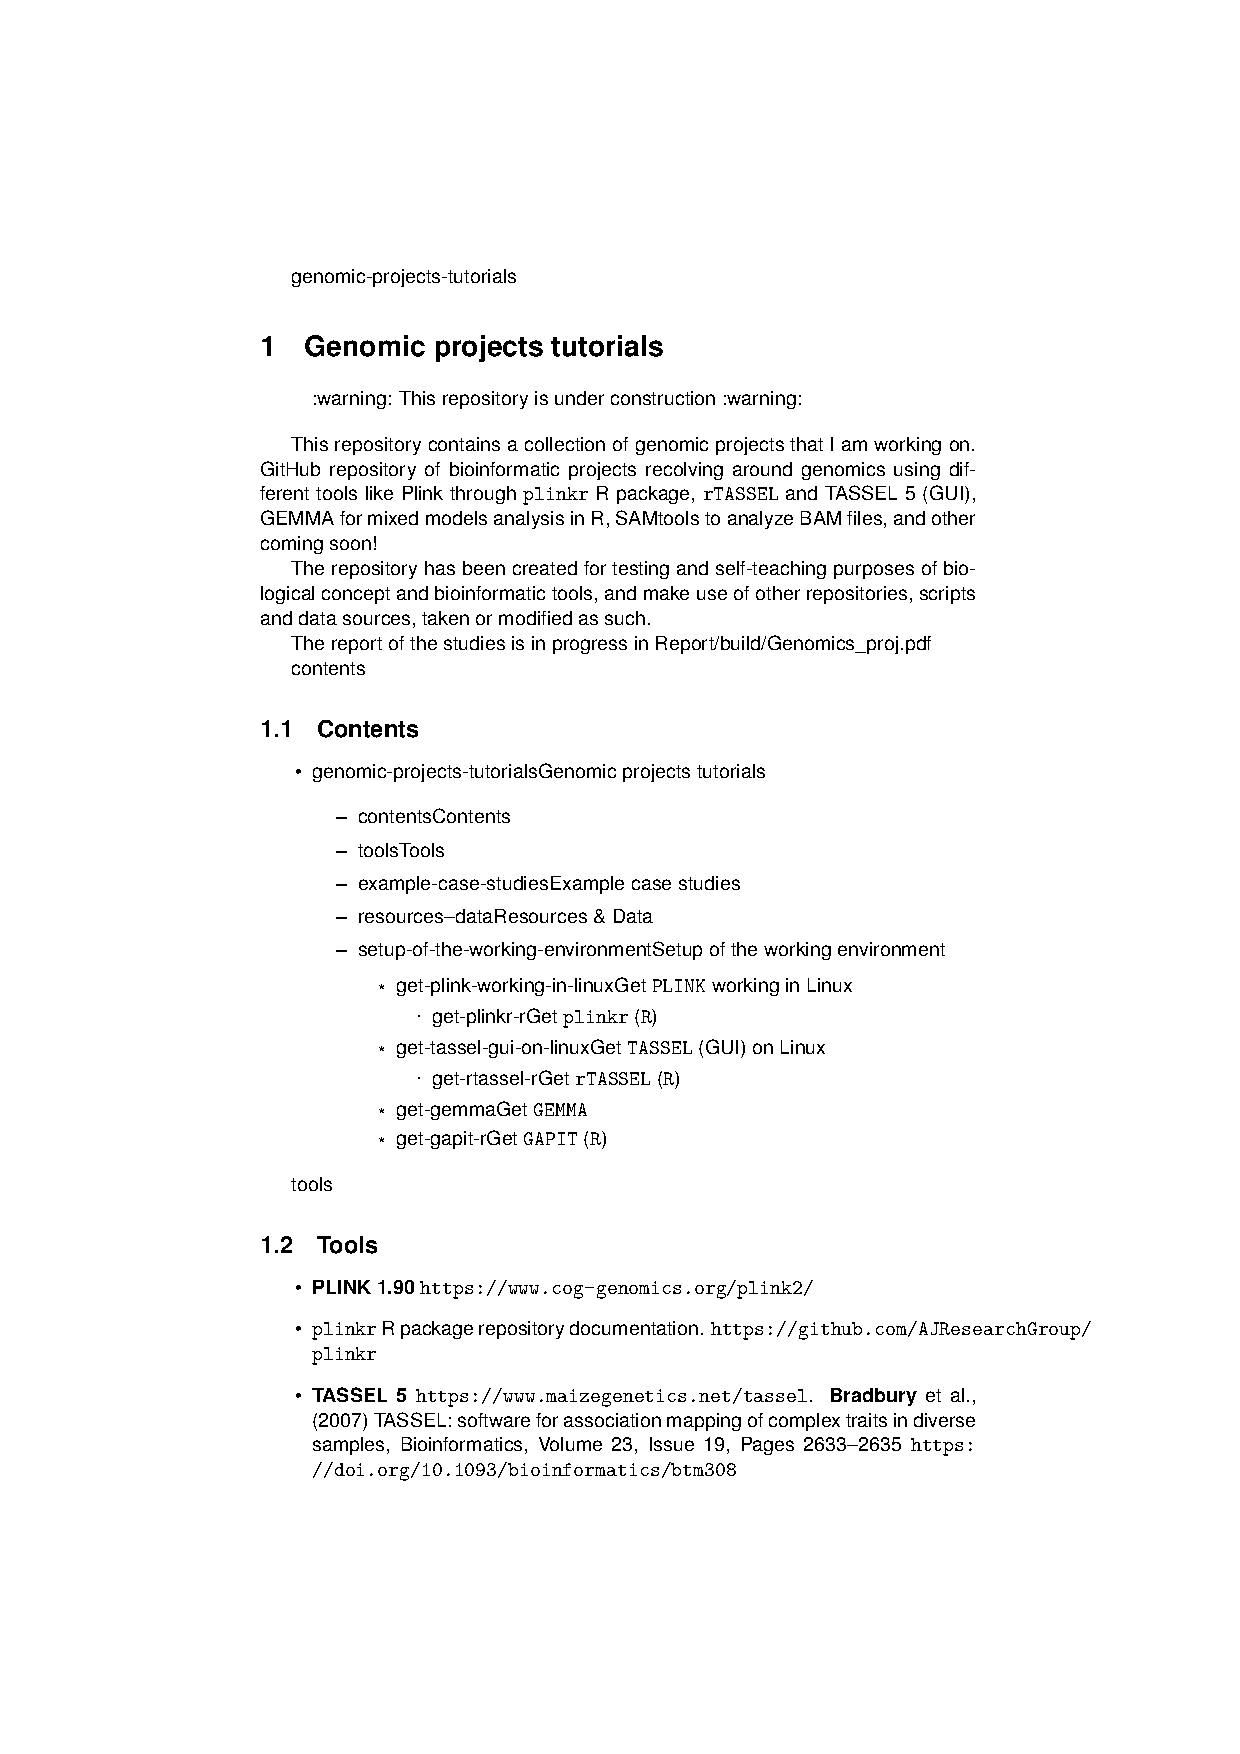
\includepdf[pages=-,pagecommand={},width=\pagewidth]{build/readme.pdf}


%\end{twocolumn}
\end{document}